\section{Introduction}

In reinforcement learning we train a model by providing it with an evaluation of its output

\paragraph*{Sequential decision making}
In the realm of sequential decision making, we navigate through a series of choices or actions aimed at achieving a specific objective. 
The optimal actions are contingent upon the context in which they occur, often lacking clear-cut examples of correctness. 
Moreover, these actions can yield long-term ramifications, and while the short-term outcomes of optimal decisions may appear unfavorable, they serve a greater purpose in the pursuit of our goals.
\begin{figure}[H]
    \centering
    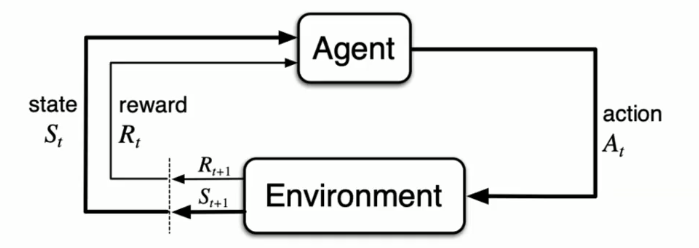
\includegraphics[width=0.75\linewidth]{images/rl.png}
    \caption{Agent-environment interface}
\end{figure}
At discrete time steps $t = 0, 1, 2, K$, the agent and environment interact as follows: the agent observes the state at step $t$, denoted as $S_t \in \mathcal{S}$, produces an action at step $t$, represented by $A_t \in \mathcal{A}(S_t)$, gets the resulting reward $R_{t+1} \in \mathcal{R}$, and transitions the environment to the next state $S_{t+1} \in \mathcal{S}$.
\begin{figure}[H]
    \centering
    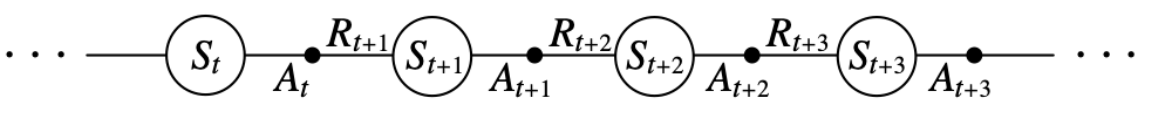
\includegraphics[width=0.75\linewidth]{images/rl1.png}
    \caption{Agent-environment interface}
\end{figure}